% vim: set spell spelllang=en tw=100 et sw=4 sts=4 foldmethod=marker foldmarker={{{,}}} :

\documentclass{beamer}

\usepackage{tikz}
\usepackage{xcolor}
\usepackage{complexity}
\usepackage{hyperref}
\usepackage{microtype}
\usepackage{amsmath}                   % \operatorname
\usepackage{amsfonts}                  % \mathcal
\usepackage{amssymb}                   % \nexists
\usepackage{gnuplot-lua-tikz}          % graphs
\usepackage[vlined]{algorithm2e} % algorithms
\usepackage{centernot}

\usetikzlibrary{shapes, arrows, shadows, calc, positioning, fit}
\usetikzlibrary{decorations.pathreplacing, decorations.pathmorphing, shapes.misc}
\usetikzlibrary{tikzmark}

\definecolor{uofguniversityblue}{rgb}{0, 0.219608, 0.396078}

\definecolor{uofgheather}{rgb}{0.356863, 0.32549, 0.490196}
\definecolor{uofgaquamarine}{rgb}{0.603922, 0.72549, 0.678431}
\definecolor{uofgslate}{rgb}{0.309804, 0.34902, 0.380392}
\definecolor{uofgrose}{rgb}{0.823529, 0.470588, 0.709804}
\definecolor{uofgmocha}{rgb}{0.709804, 0.564706, 0.47451}
\definecolor{uofgsandstone}{rgb}{0.321569, 0.278431, 0.231373}
\definecolor{uofgforest}{rgb}{0, 0.2, 0.129412}
\definecolor{uofglawn}{rgb}{0.517647, 0.741176, 0}
\definecolor{uofgcobalt}{rgb}{0, 0.615686, 0.92549}
\definecolor{uofgturquoise}{rgb}{0, 0.709804, 0.819608}
\definecolor{uofgsunshine}{rgb}{1.0, 0.862745, 0.211765}
\definecolor{uofgpumpkin}{rgb}{1.0, 0.72549, 0.282353}
\definecolor{uofgthistle}{rgb}{0.584314, 0.070588, 0.447059}
\definecolor{uofgrust}{rgb}{0.603922, 0.227451, 0.023529}
\definecolor{uofgburgundy}{rgb}{0.490196, 0.133333, 0.223529}
\definecolor{uofgpillarbox}{rgb}{0.701961, 0.047059, 0}
\definecolor{uofglavendar}{rgb}{0.356863, 0.301961, 0.580392}

\tikzset{vertex/.style={draw, circle, inner sep=0pt, minimum size=0.5cm, font=\small\bfseries}}
\tikzset{notvertex/.style={vertex, color=white, text=black}}
\tikzset{plainvertex/.style={vertex}}
\tikzset{vertexc1/.style={vertex, fill=uofgburgundy, text=white}}
\tikzset{vertexc2/.style={vertex, fill=uofgsandstone, text=white}}
\tikzset{vertexc3/.style={vertex, fill=uofgforest, text=white}}
\tikzset{vertexc4/.style={vertex, fill=uofgheather, text=white}}
\tikzset{edge/.style={color=black!50!white}}
\tikzset{bedge/.style={ultra thick}}

% {{{ theme things
\useoutertheme[footline=authortitle]{miniframes}
\useinnertheme{rectangles}

\setbeamerfont{block title}{size={}}
\setbeamerfont{title}{size=\large,series=\bfseries}
\setbeamerfont{section title}{size=\large,series=\mdseries}
\setbeamerfont{author}{size=\normalsize,series=\mdseries}
\setbeamercolor*{structure}{fg=uofguniversityblue}
\setbeamercolor*{palette primary}{use=structure,fg=black,bg=white}
\setbeamercolor*{palette secondary}{use=structure,fg=white,bg=uofgcobalt}
\setbeamercolor*{palette tertiary}{use=structure,fg=white,bg=uofguniversityblue}
\setbeamercolor*{palette quaternary}{fg=white,bg=black}

\setbeamercolor*{titlelike}{parent=palette primary}

\beamertemplatenavigationsymbolsempty

\setbeamertemplate{title page}
{
    \begin{tikzpicture}[remember picture, overlay]
        \node (shade) at (current page.north west) {
            \begin{tikzpicture}[remember picture, overlay]
                \fill [fill=white, anchor=north west, yshift=-0.5cm, opacity=0.8] (0, 0) rectangle (\paperwidth, -3.2cm);
            \end{tikzpicture}
        };

        \node [anchor=west, xshift=0.4cm, yshift=-2cm] at (shade.west) {
            \begin{minipage}{0.95\paperwidth}\raggedright
                {\usebeamerfont{title}\usebeamercolor[black]{}\inserttitle}\\[0.2cm]
                {\usebeamerfont{author}\usebeamercolor[black]{}\insertauthor}
            \end{minipage}
        };
    \end{tikzpicture}
}

\setbeamertemplate{section page}
{
    \begin{centering}
        \begin{beamercolorbox}[sep=12pt,center]{part title}
            \usebeamerfont{section title}\insertsection\par
        \end{beamercolorbox}
    \end{centering}
}

\newcommand{\frameofframes}{/}
\newcommand{\setframeofframes}[1]{\renewcommand{\frameofframes}{#1}}

\makeatletter
\setbeamertemplate{footline}
{%
    \begin{beamercolorbox}[colsep=1.5pt]{upper separation line foot}
    \end{beamercolorbox}
    \begin{beamercolorbox}[ht=2.5ex,dp=1.125ex,%
        leftskip=.3cm,rightskip=.3cm plus1fil]{author in head/foot}%
        \leavevmode{\usebeamerfont{author in head/foot}\insertshortauthor}%
        \hfill%
        {\usebeamerfont{institute in head/foot}\usebeamercolor[fg]{institute in head/foot}\insertshortinstitute}%
    \end{beamercolorbox}%
    \begin{beamercolorbox}[ht=2.5ex,dp=1.125ex,%
        leftskip=.3cm,rightskip=.3cm plus1fil]{title in head/foot}%
        {\usebeamerfont{title in head/foot}\insertshorttitle}%
        \hfill%
        {\usebeamerfont{frame number}\usebeamercolor[fg]{frame number}\insertframenumber~\frameofframes~\inserttotalframenumber}
    \end{beamercolorbox}%
    \begin{beamercolorbox}[colsep=1.5pt]{lower separation line foot}
    \end{beamercolorbox}
}

\makeatletter
\newenvironment{nearlyplainframe}[2][]{
    \def\beamer@entrycode{\vspace*{-\headheight}\vspace*{3pt}}
    \setbeamertemplate{headline}
    {%
        \begin{beamercolorbox}[colsep=1.5pt]{upper separation line head}
        \end{beamercolorbox}
        \begin{beamercolorbox}[ht=0.5ex,dp=0.125ex,%
            leftskip=.3cm,rightskip=.3cm plus1fil]{title in head/foot}%
        \end{beamercolorbox}%
        \begin{beamercolorbox}[ht=0.5ex,dp=0.125ex,%
            leftskip=.3cm,rightskip=.3cm plus1fil]{author in head/foot}%
        \end{beamercolorbox}%
        \begin{beamercolorbox}[colsep=1.5pt]{lower separation line head}
        \end{beamercolorbox}
        \vspace*{\headheight}
    }

    \setbeamertemplate{footline}
    {%
        \begin{beamercolorbox}[colsep=1.5pt]{upper separation line foot}
        \end{beamercolorbox}
        \begin{beamercolorbox}[ht=0.5ex,dp=0.125ex,%
            leftskip=.3cm,rightskip=.3cm plus1fil]{author in head/foot}%
        \end{beamercolorbox}%
        \begin{beamercolorbox}[ht=0.5ex,dp=0.125ex,%
            leftskip=.3cm,rightskip=.3cm plus1fil]{title in head/foot}%
        \end{beamercolorbox}%
        \begin{beamercolorbox}[colsep=1.5pt]{lower separation line foot}
        \end{beamercolorbox}
    }

    \begin{frame}[#1]{#2}
    }{
    \end{frame}
}
\makeatother

\makeatletter
\newenvironment{justborderframe}[2][]{
    \def\beamer@entrycode{\vspace*{-\headheight}}
    \setbeamertemplate{headline}
    {%
        \begin{beamercolorbox}[colsep=1.5pt]{upper separation line head}
        \end{beamercolorbox}
        \begin{beamercolorbox}[ht=0.5ex,dp=0.125ex,%
            leftskip=.3cm,rightskip=.3cm plus1fil]{title in head/foot}%
        \end{beamercolorbox}%
        \begin{beamercolorbox}[ht=0.5ex,dp=0.125ex,%
            leftskip=.3cm,rightskip=.3cm plus1fil]{author in head/foot}%
        \end{beamercolorbox}%
        \begin{beamercolorbox}[colsep=1.5pt]{lower separation line head}
        \end{beamercolorbox}
        \vspace*{\headheight}
    }

    \setbeamertemplate{footline}
    {%
        \begin{beamercolorbox}[colsep=1.5pt]{upper separation line foot}
        \end{beamercolorbox}
        \begin{beamercolorbox}[ht=0.5ex,dp=0.125ex,%
            leftskip=.3cm,rightskip=.3cm plus1fil]{author in head/foot}%
        \end{beamercolorbox}%
        \begin{beamercolorbox}[ht=0.5ex,dp=0.125ex,%
            leftskip=.3cm,rightskip=.3cm plus1fil]{title in head/foot}%
        \end{beamercolorbox}%
        \begin{beamercolorbox}[colsep=1.5pt]{lower separation line foot}
        \end{beamercolorbox}
    }

    \begin{frame}[#1]{}
    }{
    \end{frame}
}
\makeatother


% }}}

\author{Ruth Hoffmann \and Ciaran McCreesh \and Samba Ndojh Ndiaye \and \\ Patrick Prosser \and Craig Reilly \and Christine Solnon \and James Trimble}
\title{Observations from Parallelising Three Maximum Common (Connected) Subgraph Algorithms}

\begin{document}

{
    \usebackgroundtemplate{
        \tikz[overlay, remember picture]
        \node[at=(current page.south), anchor=south, inner sep=0pt]{\includegraphics[keepaspectratio=true, height=\paperheight]{background.jpg}};
    }
    \begin{frame}[plain,noframenumbering]
        \titlepage
    \end{frame}
}

\begin{frame}{Maximum Common Induced Subgraph}
    \centering
    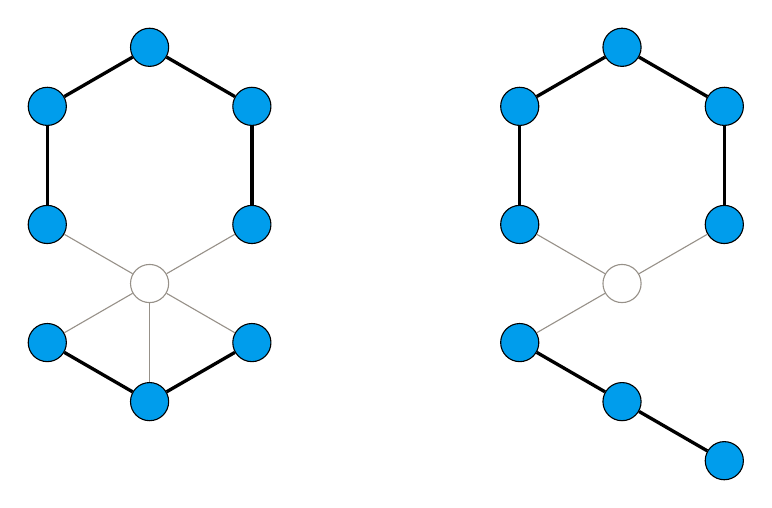
\begin{tikzpicture}
        \begin{scope}
            \node[draw, circle, fill=uofgcobalt, inner sep=2pt, font=\normalsize] (M1) at (90:1.5) {\phantom{0}};
            \node[draw, circle, fill=uofgcobalt, inner sep=2pt, font=\normalsize] (M2) at (150:1.5) {\phantom{0}};
            \node[draw, circle, fill=uofgcobalt, inner sep=2pt, font=\normalsize] (M3) at (30:1.5) {\phantom{0}};
            \node[draw, circle, fill=uofgcobalt, inner sep=2pt, font=\normalsize] (M4) at (210:1.5) {\phantom{0}};
            \node[draw, circle, fill=uofgcobalt, inner sep=2pt, font=\normalsize] (M5) at (330:1.5) {\phantom{0}};
            \node[draw, circle, draw=uofgsandstone!60, fill=white, inner sep=2pt, font=\normalsize] (M6) at (270:1.5) {\phantom{0}};
            \node[draw, circle, fill=uofgcobalt, inner sep=2pt, font=\normalsize] (M7) at ($(210:1.5) + (M6)$) {\phantom{0}};
            \node[draw, circle, fill=uofgcobalt, inner sep=2pt, font=\normalsize] (M8) at ($(330:1.5) + (M6)$) {\phantom{0}};
            \node[draw, circle, fill=uofgcobalt, inner sep=2pt, font=\normalsize] (M9) at ($(270:1.5) + (M6)$) {\phantom{0}};

            \draw [very thick] (M1) -- (M2);
            \draw [very thick] (M2) -- (M4);
            \draw [very thick] (M3) -- (M5);
            \draw [color=uofgsandstone!60] (M4) -- (M6);
            \draw [color=uofgsandstone!60] (M5) -- (M6);
            \draw [very thick] (M3) -- (M1);
            \draw [color=uofgsandstone!60] (M6) -- (M7);
            \draw [color=uofgsandstone!60] (M6) -- (M8);
            \draw [color=uofgsandstone!60] (M6) -- (M9);
            \draw [very thick] (M7) -- (M9);
            \draw [very thick] (M8) -- (M9);
        \end{scope}

        \begin{scope}[xshift=6cm]
            \node[draw, circle, fill=uofgcobalt, inner sep=2pt, font=\normalsize] (M1) at (90:1.5) {\phantom{0}};
            \node[draw, circle, fill=uofgcobalt, inner sep=2pt, font=\normalsize] (M2) at (150:1.5) {\phantom{0}};
            \node[draw, circle, fill=uofgcobalt, inner sep=2pt, font=\normalsize] (M3) at (30:1.5) {\phantom{0}};
            \node[draw, circle, fill=uofgcobalt, inner sep=2pt, font=\normalsize] (M4) at (210:1.5) {\phantom{0}};
            \node[draw, circle, fill=uofgcobalt, inner sep=2pt, font=\normalsize] (M5) at (330:1.5) {\phantom{0}};
            \node[draw, circle, draw=uofgsandstone!60, fill=white, inner sep=2pt, font=\normalsize] (M6) at (270:1.5) {\phantom{0}};
            \node[draw, circle, fill=uofgcobalt, inner sep=2pt, font=\normalsize] (M7) at ($(210:1.5) + (M6)$) {\phantom{0}};
            \node[draw, circle, fill=uofgcobalt, inner sep=2pt, font=\normalsize] (M8) at ($(270:1.5) + (M6)$) {\phantom{0}};
            \node[draw, circle, fill=uofgcobalt, inner sep=2pt, font=\normalsize] (M9) at ($(330:1.5) + (M8)$) {\phantom{0}};

            \draw [very thick] (M1) -- (M2);
            \draw [very thick] (M2) -- (M4);
            \draw [very thick] (M3) -- (M5);
            \draw [color=uofgsandstone!60] (M4) -- (M6);
            \draw [color=uofgsandstone!60] (M5) -- (M6);
            \draw [very thick] (M3) -- (M1);
            \draw [color=uofgsandstone!60] (M6) -- (M7);
            \draw [very thick] (M7) -- (M8);
            \draw [very thick] (M8) -- (M9);
        \end{scope}
    \end{tikzpicture}
\end{frame}

\begin{frame}{Maximum Common Connected Subgraph}
    \centering
    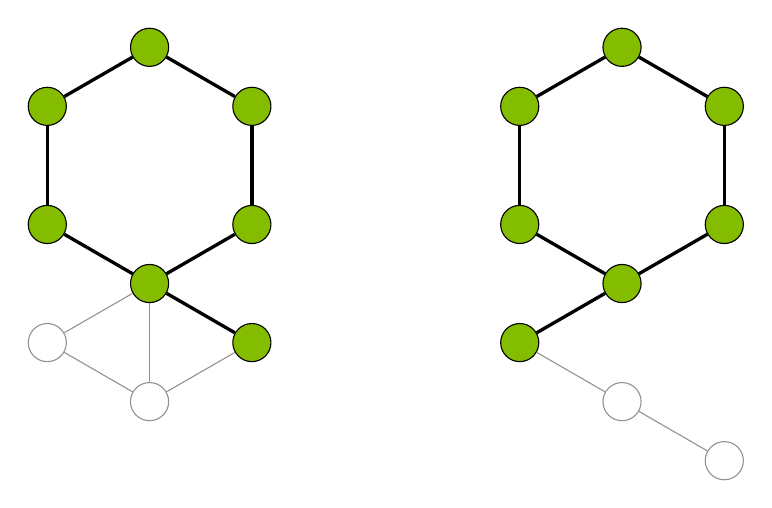
\begin{tikzpicture}
        \begin{scope}
            \node[draw, circle, fill=uofglawn, inner sep=2pt, font=\normalsize] (M1) at (90:1.5) {\phantom{0}};
            \node[draw, circle, fill=uofglawn, inner sep=2pt, font=\normalsize] (M2) at (150:1.5) {\phantom{0}};
            \node[draw, circle, fill=uofglawn, inner sep=2pt, font=\normalsize] (M3) at (30:1.5) {\phantom{0}};
            \node[draw, circle, fill=uofglawn, inner sep=2pt, font=\normalsize] (M4) at (210:1.5) {\phantom{0}};
            \node[draw, circle, fill=uofglawn, inner sep=2pt, font=\normalsize] (M5) at (330:1.5) {\phantom{0}};
            \node[draw, circle, fill=uofglawn, inner sep=2pt, font=\normalsize] (M6) at (270:1.5) {\phantom{0}};
            \node[draw, circle, draw=uofgsandstone!60, fill=white, inner sep=2pt, font=\normalsize] (M7) at ($(210:1.5) + (M6)$) {\phantom{0}};
            \node[draw, circle, fill=uofglawn, inner sep=2pt, font=\normalsize] (M8) at ($(330:1.5) + (M6)$) {\phantom{0}};
            \node[draw, circle, draw=uofgsandstone!60, fill=white, inner sep=2pt, font=\normalsize] (M9) at ($(270:1.5) + (M6)$) {\phantom{0}};

            \draw [very thick] (M1) -- (M2);
            \draw [very thick] (M2) -- (M4);
            \draw [very thick] (M3) -- (M5);
            \draw [very thick] (M4) -- (M6);
            \draw [very thick] (M5) -- (M6);
            \draw [very thick] (M3) -- (M1);
            \draw [color=uofgsandstone!60] (M6) -- (M7);
            \draw [very thick] (M6) -- (M8);
            \draw [color=uofgsandstone!60] (M6) -- (M9);
            \draw [color=uofgsandstone!60] (M7) -- (M9);
            \draw [color=uofgsandstone!60] (M8) -- (M9);
        \end{scope}

        \begin{scope}[xshift=6cm]
            \node[draw, circle, fill=uofglawn, inner sep=2pt, font=\normalsize] (M1) at (90:1.5) {\phantom{0}};
            \node[draw, circle, fill=uofglawn, inner sep=2pt, font=\normalsize] (M2) at (150:1.5) {\phantom{0}};
            \node[draw, circle, fill=uofglawn, inner sep=2pt, font=\normalsize] (M3) at (30:1.5) {\phantom{0}};
            \node[draw, circle, fill=uofglawn, inner sep=2pt, font=\normalsize] (M4) at (210:1.5) {\phantom{0}};
            \node[draw, circle, fill=uofglawn, inner sep=2pt, font=\normalsize] (M5) at (330:1.5) {\phantom{0}};
            \node[draw, circle, fill=uofglawn, inner sep=2pt, font=\normalsize] (M6) at (270:1.5) {\phantom{0}};
            \node[draw, circle, fill=uofglawn, inner sep=2pt, font=\normalsize] (M7) at ($(210:1.5) + (M6)$) {\phantom{0}};
            \node[draw, circle, draw=uofgsandstone!60, fill=white, inner sep=2pt, font=\normalsize] (M8) at ($(270:1.5) + (M6)$) {\phantom{0}};
            \node[draw, circle, draw=uofgsandstone!60, fill=white, inner sep=2pt, font=\normalsize] (M9) at ($(330:1.5) + (M8)$) {\phantom{0}};

            \draw [very thick] (M1) -- (M2);
            \draw [very thick] (M2) -- (M4);
            \draw [very thick] (M3) -- (M5);
            \draw [very thick] (M4) -- (M6);
            \draw [very thick] (M5) -- (M6);
            \draw [very thick] (M3) -- (M1);
            \draw [very thick] (M6) -- (M7);
            \draw [draw=uofgsandstone!60] (M7) -- (M8);
            \draw [draw=uofgsandstone!60] (M8) -- (M9);
        \end{scope}
    \end{tikzpicture}
\end{frame}

\begin{frame}{Maximum Common Subgraph Problems are Hard}
    \begin{itemize}
        \item State of the art can struggle with:
            \begin{itemize}
                \item 50 vertices on unlabelled graphs (two years ago: 35 vertices).
                \item 100 vertices on labelled graphs (two years ago: 50 vertices).
            \end{itemize}
        \item If the solution is nearly all of the smaller of the two graphs, the problem is easier
            and we can approach ten thousand vertices in the larger graph.
    \end{itemize}
\end{frame}

\begin{frame}{CP Models}
    \begin{itemize}
        \item One variable for each vertex in the smaller input graph.
        \item Domains range over vertices in the other input graph, plus $\bot$.
        \item Objective is to maximise variables not assigned $\bot$.
        \item Adjacent pairs of non-$\bot$ vertices must be mapped to adjacent pairs of vertices.
        \item Non-adjacent pairs of non-$\bot$ vertices must be mapped to non-adjacent pairs of vertices.
        \item All different except $\bot$, with number of allowed $\bot$ occurrences controlled by
            the objective variable.
        \item Smallest domain first, prefer vertices of similar degree.
    \end{itemize}
\end{frame}

\begin{frame}{McSplit and McSplit{$\downarrow$} (IJCAI 2017)}
    \begin{itemize}
        \item During search, any two domains are either identical or disjoint, excluding $\bot$.
        \item Backtrackable partition data structures.
        \item Can propagate the bound in linear time.
        \item Can do dual viewpoint variable and value ordering heuristics in linear time and no
            extra space.
        \item Two variants: conventional branch and bound, or descending.
    \end{itemize}
\end{frame}

\begin{frame}{k{$\downarrow$} (AAAI 2017)}
    \begin{itemize}
        \item Start by trying to find an induced subgraph isomorphism.
        \item If that fails, try again allowing one wildcard.
        \item Then two wildcards, and so on.
        \item CP-like algorithm with special data structures.
    \end{itemize}
\end{frame}

\begin{frame}{Clique Models and Microstructure (CP 2016)}
    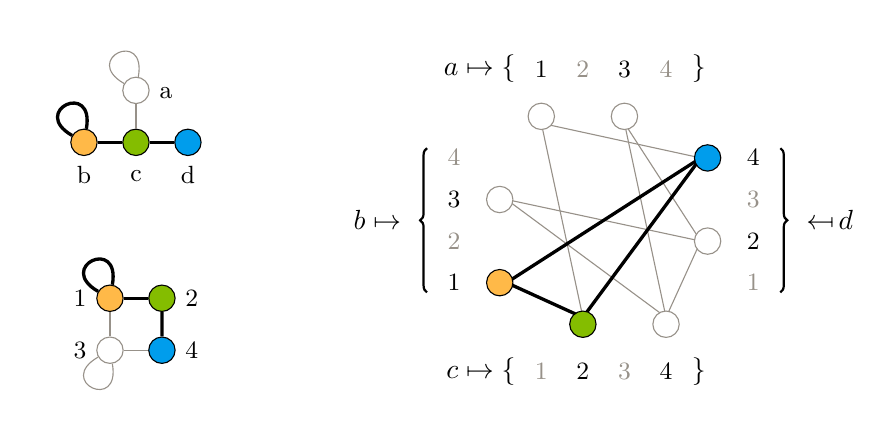
\begin{tikzpicture}[scale=0.33]%{{{
        \begin{scope}
            \node[draw, circle, fill=white, draw=uofgsandstone!60, inner sep=0.5pt, font=\normalsize] (Ma) at (2, 8) {\phantom{0}};
            \node[draw, circle, fill=uofgpumpkin, inner sep=0.5pt, font=\normalsize] (Mb) at (0, 6) {\phantom{0}};
            \node[draw, circle, fill=uofglawn, inner sep=0.5pt, font=\normalsize] (Mc) at (2, 6) {\phantom{0}};
            \node[draw, circle, fill=uofgcobalt, inner sep=0.5pt, font=\normalsize] (Md) at (4, 6) {\phantom{0}};

            \node [right = 0 of Ma, font=\small] { \vphantom{0}a };
            \node [below = 0 of Mb, font=\small] { \vphantom{0}b };
            \node [below = 0 of Mc, font=\small] { \vphantom{0}c };
            \node [below = 0 of Md, font=\small] { \vphantom{0}d };

            \draw [very thick] (Mb) -- (Mc);
            \draw [very thick] (Mc) -- (Md);
            \draw [color=uofgsandstone!60] (Ma) -- (Mc);
            \draw [color=uofgsandstone!60] (Ma) to [out=150, in=80, looseness=8] (Ma);
            \draw [very thick] (Mb) to [out=150, in=80, looseness=8] (Mb);
        \end{scope}

        \begin{scope}[yshift=-2cm]
            \node[draw, circle, fill=uofgpumpkin, inner sep=0.5pt, font=\normalsize] (M1) at (1, 2) {\phantom{0}};
            \node[draw, circle, fill=uofglawn, inner sep=0.5pt, font=\normalsize] (M2) at (3, 2) {\phantom{0}};
            \node[draw, circle, fill=white, draw=uofgsandstone!60, inner sep=0.5pt, font=\normalsize] (M3) at (1, 0) {\phantom{0}};
            \node[draw, circle, fill=uofgcobalt, inner sep=0.5pt, font=\normalsize] (M4) at (3, 0) {\phantom{0}};

            \node [left = 0 of M1, font=\small] { \vphantom{0}1 };
            \node [right = 0 of M2, font=\small] { \vphantom{0}2 };
            \node [left = 0 of M3, font=\small] { \vphantom{0}3 };
            \node [right = 0 of M4, font=\small] { \vphantom{0}4 };

            \draw [very thick] (M1) -- (M2);
            \draw [very thick] (M2) -- (M4);
            \draw [color=uofgsandstone!60] (M3) -- (M4);
            \draw [color=uofgsandstone!60] (M1) -- (M3);

            \draw [color=uofgsandstone!60] (M3) to [out=280, in=210, looseness=8] (M3);
            \draw [very thick] (M1) to [out=150, in=80, looseness=8] (M1);
        \end{scope}

        \begin{scope}[xshift=15cm, yshift=-2cm]
            \node[draw, circle, fill=white, draw=uofgsandstone!60, inner sep=0.5pt, font=\normalsize] (Ma1) at (2.6, 9) {\phantom{0}};
            \node[draw, circle, fill=white, draw=white, inner sep=0.5pt, font=\normalsize] (Ma2) at (4.2, 9) {\phantom{0}};
            \node[draw, circle, fill=white, draw=uofgsandstone!60, inner sep=0.5pt, font=\normalsize] (Ma3) at (5.8, 9) {\phantom{0}};
            \node[draw, circle, fill=white, draw=white, inner sep=0.5pt, font=\normalsize] (Ma4) at (7.4, 9) {\phantom{0}};
            \node (La1) [above = 0.2cm of Ma1, font=\small] { \vphantom{0}1 };
            \node (La2) [above = 0.2cm of Ma2, font=\small, color=uofgsandstone!60] { \vphantom{0}2 };
            \node (La3) [above = 0.2cm of Ma3, font=\small] { \vphantom{0}3 };
            \node (La4) [above = 0.2cm of Ma4, font=\small, color=uofgsandstone!60] { \vphantom{0}4 };

            \node [left=0 of La1] { $a \mapsto \{$ };
            \node [right=0 of La4] { $\}$ };

            \node[draw, circle, fill=uofgpumpkin, inner sep=0.5pt, font=\normalsize] (Mb1) at (1, 2.6) {\phantom{0}};
            \node[draw, circle, fill=white, draw=white, inner sep=0.5pt, font=\normalsize] (Mb2) at (1, 4.2) {\phantom{0}};
            \node[draw, circle, fill=white, draw=uofgsandstone!60, inner sep=0.5pt, font=\normalsize] (Mb3) at (1, 5.8) {\phantom{0}};
            \node[draw, circle, fill=white, draw=white, inner sep=0.5pt, font=\normalsize] (Mb4) at (1, 7.4) {\phantom{0}};
            \node [left = 0.2cm of Mb1, font=\small] { \vphantom{0}1 };
            \node [left = 0.2cm of Mb2, font=\small, color=uofgsandstone!60] { \vphantom{0}2 };
            \node [left = 0.2cm of Mb3, font=\small] { \vphantom{0}3 };
            \node [left = 0.2cm of Mb4, font=\small, color=uofgsandstone!60] { \vphantom{0}4 };

            \draw [decorate, decoration={brace, raise=0.8cm}, thick] (Mb1.south west) -- (Mb4.north west) node [midway, left=1cm] { $b \mapsto$ };

            \node[draw, circle, fill=white, draw=white, inner sep=0.5pt, font=\normalsize] (Mc1) at (2.6, 1) {\phantom{0}};
            \node[draw, circle, fill=uofglawn, inner sep=0.5pt, font=\normalsize] (Mc2) at (4.2, 1) {\phantom{0}};
            \node[draw, circle, fill=white, draw=white, inner sep=0.5pt, font=\normalsize] (Mc3) at (5.8, 1) {\phantom{0}};
            \node[draw, circle, fill=white, draw=uofgsandstone!60, inner sep=0.5pt, font=\normalsize] (Mc4) at (7.4, 1) {\phantom{0}};
            \node (Lc1) [below = 0.2cm of Mc1, font=\small, color=uofgsandstone!60] { \vphantom{0}1 };
            \node (Lc2) [below = 0.2cm of Mc2, font=\small] { \vphantom{0}2 };
            \node (Lc3) [below = 0.2cm of Mc3, font=\small, color=uofgsandstone!60] { \vphantom{0}3 };
            \node (Lc4) [below = 0.2cm of Mc4, font=\small] { \vphantom{0}4 };

            \node [left=0 of Lc1] { $c \mapsto \{$ };
            \node [right=0 of Lc4] { $\}$ };

            \node[draw, circle, fill=white, draw=white, inner sep=0.5pt, font=\normalsize] (Md1) at (9, 2.6) {\phantom{0}};
            \node[draw, circle, fill=white, draw=uofgsandstone!60, inner sep=0.5pt, font=\normalsize] (Md2) at (9, 4.2) {\phantom{0}};
            \node[draw, circle, fill=white, draw=white, inner sep=0.5pt, font=\normalsize] (Md3) at (9, 5.8) {\phantom{0}};
            \node[draw, circle, fill=uofgcobalt, inner sep=0.5pt, font=\normalsize] (Md4) at (9, 7.4) {\phantom{0}};
            \node [right = 0.2cm of Md1, font=\small, color=uofgsandstone!60] { \vphantom{0}1 };
            \node [right = 0.2cm of Md2, font=\small] { \vphantom{0}2 };
            \node [right = 0.2cm of Md3, font=\small, color=uofgsandstone!60] { \vphantom{0}3 };
            \node [right = 0.2cm of Md4, font=\small] { \vphantom{0}4 };

            \draw [decorate, decoration={brace, raise=0.8cm}, thick] (Md4.north east) -- (Md1.south east) node [midway, right=1cm] { $\reflectbox{\ensuremath{\mapsto}}\, d$ };

            \begin{scope}[on background layer]
                \draw [draw=uofgsandstone!60] ($(Ma1.south)!0.5!(Ma1)$) -- ($(Md4.west)!0.5!(Md4)$);
                \draw [draw=uofgsandstone!60] ($(Ma1.south)!0.5!(Ma1)$) -- ($(Mc2.north)!0.5!(Mc2)$);
                \draw [draw=uofgsandstone!60] ($(Ma3.south)!0.5!(Ma3)$) -- ($(Mc4.north)!0.5!(Mc4)$);
                \draw [draw=uofgsandstone!60] ($(Mb3.east)!0.5!(Mb3)$) -- ($(Mc4.north)!0.5!(Mc4)$);
                \draw [draw=uofgsandstone!60] ($(Md2.west)!0.5!(Md2)$) -- ($(Mc4.north)!0.5!(Mc4)$);
                \draw [draw=uofgsandstone!60] ($(Md2.west)!0.5!(Md2)$) -- ($(Ma3.south)!0.5!(Ma3)$);
                \draw [draw=uofgsandstone!60] ($(Md2.west)!0.5!(Md2)$) -- ($(Mb3.east)!0.5!(Mb3)$);
                \draw [very thick] ($(Mb1.east)!0.5!(Mb1)$) -- ($(Mc2.north)!0.5!(Mc2)$);
                \draw [very thick] ($(Mb1.east)!0.5!(Mb1)$) -- ($(Md4.west)!0.5!(Md4)$);
                \draw [very thick] ($(Mc2.north)!0.5!(Mc2)$) -- ($(Md4.west)!0.5!(Md4)$);
        \end{scope}
        \end{scope}

    \end{tikzpicture}
\end{frame}

\begin{frame}{Connected?}
    \begin{itemize}
        \item We can express connectivity as a constraint, or by a special branching rule.
        \item This also works inside the clique algorithm.
    \end{itemize}
\end{frame}

\begin{frame}{Parallel Tree-Search}
    \begin{itemize}
        \item All three state of the art approaches use backtracking search in some form.
        \item The search trees are particularly nasty, from a parallelism perspective:
            \begin{itemize}
                \item We have a very good value-ordering heuristic.
                \item No pruning at the top of search, and awkward changes to domain sizes during
                    search.
                \item If we have found a large solution, the optimality proof is very short.
            \end{itemize}
        \item Various attempts at static decomposition have failed miserably.
    \end{itemize}
\end{frame}

\begin{frame}{Deterministic Heuristic-Aware Work-Stealing}
    \begin{itemize}
        \item We can adapt a parallel work-stealing strategy used by the clique algorithm:
            \begin{itemize}
                \item Queue the first level of the search tree, preserving left to right ordering
                    (respecting the value-ordering heuristic).
                \item When we run out of work, re-queue remaining work at depth two.
                \item And so on.
            \end{itemize}
        \item Various nice properties, in theory:
            \begin{itemize}
                \item Respects value-ordering heuristic.
                \item Parallel can never be worse than sequential, and adding threads cannot hurt.
                \item Reproducible.
                \item Queue cannot get too big.
            \end{itemize}
    \end{itemize}
\end{frame}

\begin{frame}{Experiments}
    \begin{itemize}
        \item Dual Intel Xeon E5-2697A v4, 32 cores in total, 512GBytes RAM, Ubuntu 17.04.
        \item C++ native threads, manual work-stealing.
        \item Speedups over unmodified sequential algorithms.
        \item Standard benchmark instances:
            \begin{itemize}
                \item 4,110 small unlabelled instances of up to 50 vertices.
                \item 8,140 labelled instances of up to 100 vertices.
                \item 5,725 large unlabelled instances with differing pattern and target sizes.
            \end{itemize}
    \end{itemize}
\end{frame}

\begin{justborderframe}[t]{Cumulative Plots?}
    \includegraphics{gen-graph-cumulative-plain.pdf}\hfill\includegraphics{gen-graph-cumulative-sip.pdf}\\[10pt]
    \includegraphics{gen-graph-cumulative-33ved.pdf}\hfill\includegraphics{gen-graph-cumulative-33ve-connected.pdf}
\end{justborderframe}

\begin{justborderframe}[t]{Scatter Plots?}
    \vspace*{10pt}
    \includegraphics{gen-graph-scatter-plain-clique-vs-clique-par-t32.pdf}\hfill%
    \includegraphics{gen-graph-scatter-sip-kdown-vs-kdown-par-t32.pdf}\hfill%
    \includegraphics{gen-graph-scatter-sip-mcsplit-vs-mcsplit-par-t32.pdf} \\[10pt]
    \includegraphics{gen-graph-scatter-33ved-clique-vs-clique-par-t32.pdf}\hfill%
    \includegraphics{gen-graph-scatter-33ve-connected-clique-vs-clique-par-t32.pdf}\hfill%
    \includegraphics{gen-graph-scatter-33ve-connected-mcsplit-vs-mcsplit-par-t32.pdf}
\end{justborderframe}

\begin{nearlyplainframe}[t]{What's The Speedup?}
    \includegraphics{gen-graph-histogram-33v-clique-vs-clique-par-t32.pdf}
    \includegraphics{gen-graph-histogram-33ve-connected-clique-vs-clique-par-t32.pdf}
    \includegraphics{gen-graph-histogram-33ved-clique-vs-clique-par-t32.pdf}
    \includegraphics{gen-graph-histogram-plain-clique-vs-clique-par-t32.pdf}
    \includegraphics{gen-graph-histogram-plain-connected-clique-vs-clique-par-t32.pdf}

    \begin{itemize}
        \item Only including items with a sequential runtime of at least 500 milliseconds, that did
            not timeout\ldots
    \end{itemize}
\end{nearlyplainframe}

\begin{nearlyplainframe}[t]{Performance Profiles?}
    \includegraphics{gen-graph-pp2-33v-clique-vs-clique-par-t32.pdf}
    \includegraphics{gen-graph-pp2-33ve-connected-clique-vs-clique-par-t32.pdf}
    \includegraphics{gen-graph-pp2-33ved-clique-vs-clique-par-t32.pdf}
    \includegraphics{gen-graph-pp2-plain-clique-vs-clique-par-t32.pdf}
    \includegraphics{gen-graph-pp2-plain-connected-clique-vs-clique-par-t32.pdf}

    \begin{itemize}
        \item Heavily dependent upon how we treat sequential timeouts, and on whether we include
            trivial instances.
    \end{itemize}
\end{nearlyplainframe}

\begin{nearlyplainframe}[t]{Aggregate Speedups?}
    \includegraphics<1>{gen-graph-as-clique.pdf}
    \includegraphics<2>{gen-graph-as-kdown.pdf}
    \includegraphics<3>{gen-graph-as-mcsplit.pdf}

    \begin{itemize}
        \item Looking at the cumulative plots, how long did it take sequentially to solve the number
            of instances we can solve in this time in parallel?
    \end{itemize}
\end{nearlyplainframe}

\begin{frame}[t]{Reproducibility}
    \includegraphics{gen-graph-scatter-33ved-clique-par-t32r-vs-clique-par-t32.pdf}\hfill
    \includegraphics{gen-graph-scatter-plain-kdown-par-t32r-vs-kdown-par-t32.pdf}\hfill
    \includegraphics{gen-graph-scatter-plain-mcsplit-par-t32r-vs-mcsplit-par-t32.pdf}

    \begin{itemize}
        \item In theory, if we run the same instance twice on the same hardware, the runtimes should
            be identical.
        \item This does not happen in practice if we use conventional randomised work stealing.
    \end{itemize}
\end{frame}

\begin{frame}[t]{Scalability}
    \includegraphics{gen-graph-scatter-33ved-clique-par-t2-vs-clique-par-t4.pdf}\hfill%
    \includegraphics{gen-graph-scatter-33ved-clique-par-t4-vs-clique-par-t8.pdf}\hfill%
    \includegraphics{gen-graph-scatter-33ved-clique-par-t8-vs-clique-par-t16.pdf}

    \begin{itemize}
        \item In theory, increasing the number of threads cannot make things worse.
    \end{itemize}
\end{frame}

\begin{frame}{Conclusion}
    \begin{itemize}
        \item Parallel is better than sequential.
        \item But it is very sensitive to both instance and algorithm choice.
        \item Evaluating parallel algorithms is hard.
    \end{itemize}
\end{frame}

\begin{justborderframe}[t,noframenumbering]{}
    \begin{center}
        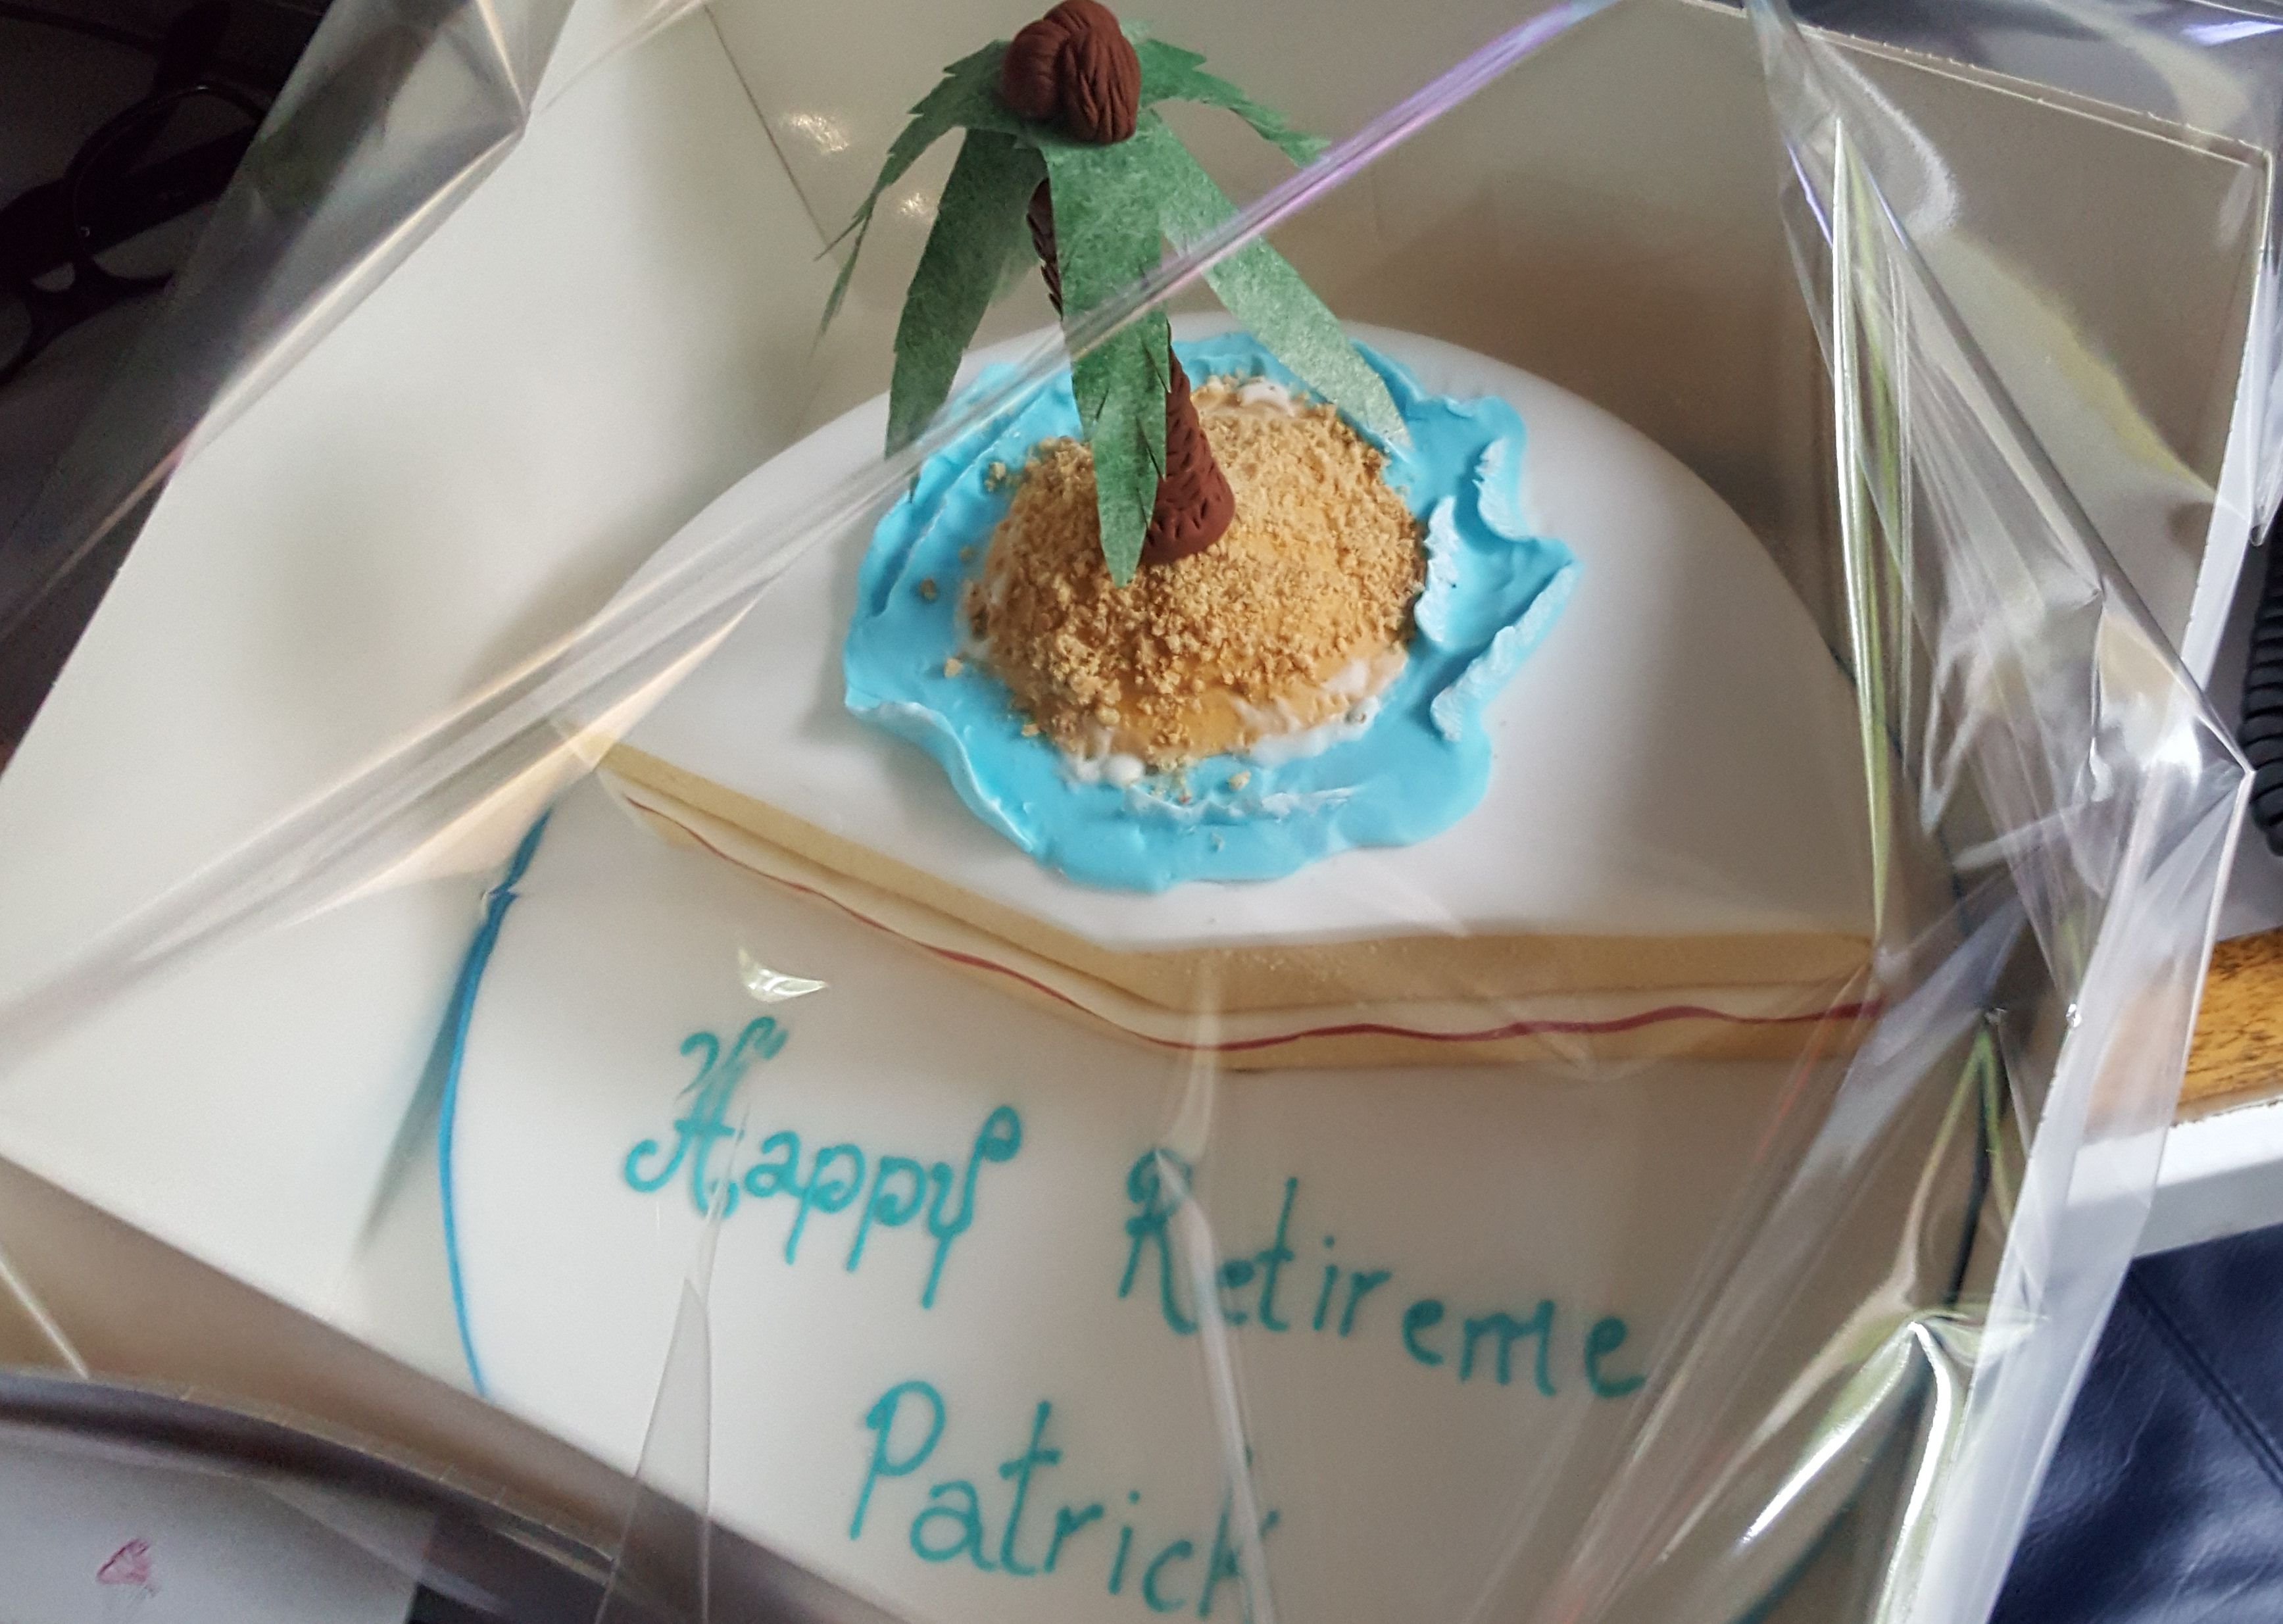
\includegraphics[keepaspectratio=true,width=0.6\paperwidth]{cake.jpg} \\
        \vspace*{4em}
        \url{http://www.dcs.gla.ac.uk/~ciaran} \\
        \href{mailto:ciaran.mccreesh@glasgow.ac.uk}{\nolinkurl{ciaran.mccreesh@glasgow.ac.uk}} \\
    \end{center}
\end{justborderframe}

\end{document}

